\documentclass{article}

\usepackage{ctex}
\usepackage{listings}
\usepackage[framed,numbered,autolinebreaks,useliterate]{mcode}
\usepackage{geometry}
\usepackage{multirow}
\usepackage{graphicx}
\usepackage{amsmath}
\usepackage{float}
\geometry{a4paper, scale=0.8}

\title{数学实验实验报告}
\author{ZhaohengLi 2017050025\\cainetatum@foxmail.com\\15801206130}

\begin{document}
\maketitle
\section{实验目的}
\begin{itemize}
	\item{掌握用MATLAB软件求解非线性方程和方程组的基本用法,并对结果作初步分析。}
	\item{练习用非线性方程和方程组建立实际问题的模型并进行求解。}
\end{itemize}

\newpage
\section{CH6-T3 贷款}

\subsection{(1)}
\subsubsection{模型建立}
设$x_k$为第k个月的欠款数,a为月还款数,r为月利率,由此我们得到迭代关系式:
$$x_{k+1}=(1+r)*x_k-a$$

多次迭代可以得到:
$$x_k=(1+r)^k*x_0-a*\frac{(1+r)^k-1}{r}$$

MATLAB代码如下:

\begin{lstlisting}
%% Global Variables
x0 = 15; % 借款总额
a = 0.1; % 每月还款额
k = 15; % 还清年限

%% Cal
init = 0.1;
r = fzero(@rate,init,[],x0,a,k,1)

%% Func
function y = rate(r,x0,a,k,byMonth)
    if (byMonth)
        y = (1+r)^(k*12)*x0-a*((1+r)^(k*12)-1)/r;
    else
        y = (1+r)^k*x0-a*((1+r)^k-1)/r;
    end
end

\end{lstlisting}

\subsubsection{计算结果}
根据$a=0.1,x_0=15,x_{180}=0$解得$r=0.0020811$,即月利率约为0.21\%,通过变换初值以及设置精度的检验,该结果较为精确。

\subsection{(2)}
本小题的模型依旧与第一小题相同。

MATLAB代码如下:
\begin{lstlisting}
%% Global Variables
x0 = 50; % 借款总额
a1 = 0.45; % 每月还款额
a2 = 4.5;
k1 = 15; % 还清年限
k2 = 20;
%% Cal
init = 0.1;
r1 = fzero(@rate,init,[],x0,a1,k1,1)*12
r2 = fzero(@rate,init,[],x0,a2,k2,0)

%% Func
function y = rate(r,x0,a,k,byMonth)
    if (byMonth)
        y = (1+r)^(k*12)*x0-a*((1+r)^(k*12)-1)/r;
    else
        y = (1+r)^k*x0-a*((1+r)^k-1)/r;
    end
end
\end{lstlisting}

解得$r_1=0.0702,r_2=0.0639$,即第一家银行的年利率为7.02\%,第二家银行的年利率为6.36\%,所以第二家银行的利率比较低。

\section{CH6-T6 均相共沸混合物}
\subsection{模型建立与算法设计}
基本建立模型同例题,设$x_i$为第$i$种组分的占比,$T$为温度,则对于该系统,有下列方程成立:

\begin{figure}[H]
    \centering
    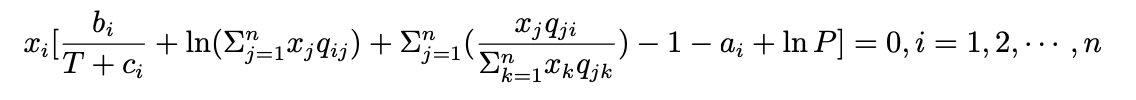
\includegraphics[width=0.7\textwidth]{pic1.png}
\end{figure}

在实际进行求解的时候,利用共沸物组分之和为 $1$ 的条件有:

$$x_n = 1-\sum_{i=1}^{n-1}x_i$$

可以列出关于$x_1,\cdots,x_{n-1},T$的n个非线性方程组,该方程组难以求得解析解,因此使用MATLAB中的$fslove()$求解。

MATLAB代码如下:
\begin{lstlisting}
%% Global Variables
n = 4;
P = 760;
a = [18.607, 15.841, 20.443, 19.293]';
b = [3643.31, 2755.64, 4628.96, 4117.07]';
c = [239.73, 219.16, 252.64, 227.44]';
Q = [1.0 0.192 2.169 1.611;
     0.316 1.0 0.477 0.524;
     0.377 0.360 1.0 0.296;
     0.524 0.282 2.065 1.0];
XT0 = [0.25, 0.25, 0.25, 100]';
[XT,Y]=fsolve(@azeofun,XT0,[],n,P,a,b,c,Q);

%% Func
function f=azeofun(XT,n,P,a,b,c,Q)
x(n)=1;
for i=1:n-1
    x(i)=XT(i);
    x(n)=x(n)-x(i);
end
T=XT(n);
p=log(P);
for i=1:n
   d(i) = x * Q(i,1:n)';
   dd(i)=x(i)/d(i);
end
for i=1:n
    f(i)=x(i)*(b(i)/(T+c(i)) + log(x*Q(i,1:n)') + dd*Q(1:n,i) - a(i) - 1 + p);
end
end
\end{lstlisting}

\subsection{计算结果}
通过多次改变初值发现,该方程组对于温度的变化较为敏感,因此接下来的初值设置重点在于温度的改变。

当初值为$[0.25,0.25,0.25,10/20/30/40/50/60/65]$这七组数据时,能够解出:
$$x_1=62.47\%,x_2=37.53\%,x_3=0.00\%,x_4=0.00\%,T=58.1358$$

当初值为$[0.05,0.2,0.6,10/20/30/40/50/60/65]$这七组数据时,能够解出:
$$x_1=62.47\%,x_2=37.53\%,x_3=0.00\%,x_4=0.00\%,T=58.1358$$

当初值为$[0.25,0.25,0.25,70/75]$这两组数据时,能够解出:
$$x_1=0.00\%,x_2=58.58\%,x_3=41.42\%,x_4=0.00\%,T=71.9657$$

当初值为$[0.2,0.33,0.33,70/75]$这两组数据时,能够解出:
$$x_1=0.00\%,x_2=58.58\%,x_3=41.42\%,x_4=0.00\%,T=71.9657$$

当初值为$[0.0,0.7,0,76]$这两组数据时,能够解出:
$$x_1=0.00\%,x_2=78.03\%,x_3=0.00\%,x_4=21.97\%,T=76.9613$$

当初值为$[0.25,0.25,0.25,80/85]$这两组数据时,能够解出:
$$x_1=0.00\%,x_2=0.00\%,x_3=100\%,x_4=0.00\%,T=82.5567$$

当初值为$[0.25,0.25,0.25,90/95/100/110]$这四组数据时,能够解出:
$$x_1=0.00\%,x_2=0.00\%,x_3=0.00\%,x_4=100\%,T=97.7712$$

\subsection{结果分析与结论}

可以看出,在找出的几组解中,没有出现所有的$x_i$均大于0的情况,这四种物质可能 不能共同稳定存在。又由共沸物的定义,必须由一种以上的物质,上述几种情况中有些仅仅有一种物质存在(其他物质的成分占比均为0.00\%),不符合定义。

综上所述,最终符合条件的物质配比和温度为:

$$x_1=62.47\%,x_2=37.53\%,x_3=0.00\%,x_4=0.00\%,T=58.1358$$

$$x_1=0.00\%,x_2=58.58\%,x_3=41.42\%,x_4=0.00\%,T=71.9657$$

$$x_1=0.00\%,x_2=78.03\%,x_3=0.00\%,x_4=21.97\%,T=76.9613$$

\section{CH6-T8 商品}
\subsection{模型建立与算法设计}
根据商品供求关系,可以得出期望价格 q 的递推公式为:
$$q_{t+1} = \frac{r}{d}[c-arctan(\mu q_t)]-(r-1)q_t$$

为了观察混沌现象并计算分岔点,可以采用课本中提供的chaos函数画出分岔图进行观察分岔点的大致位置。

找到大概位置后,再通过设置计算区间,使用枚举的方式确定分岔点的精确位置,即计算出现两倍于原来个收敛序列的起始点即可。

MATLAB代码如下:
\begin{lstlisting}
%% Global Variables
init_val = 0.5;
chaos(@qt, init_val, [0, 2, 0.001], [1000, 1200]);
%% Find Fork Point
search(@qt, init_val, 1000, 1.0:0.0001:1.1, 0, 1e-7)
%% Func
function [y] = qt(x,c)
y = 0.3/0.25*(c-atan(4.8*x))-(0.3-1)*x;
end

function chaos(iter_fun, x0, r, n)
    kr = 0;
    for rr = r(1):r(3):r(2)
        kr = kr + 1;
        y(kr, 1) = feval(iter_fun, x0, rr);
        for i = 2:n(2)
            y(kr,i) = feval(iter_fun, y(kr, i - 1), rr);
        end
    end
    plot([r(1):r(3):r(2)], y(:, n(1) + 1: n(2)), 'k.');
end

function [fp] = search(iter_fun, init_val, converge_iter, search_range, level, tol)
    fp = -1;
    for c = search_range
        iter_val = init_val;
        for i = 1:converge_iter
            iter_val = feval(iter_fun, iter_val, c);
        end
        sample_count = 2 ^ (level + 1);
        sample_vector = zeros(sample_count, 1);
        for i = 1:sample_count
            sample_vector(i) = feval(iter_fun, iter_val, c);
            iter_val = sample_vector(i);
        end
        converge_mat = reshape(sample_vector, [], 2);
        converge_mat = abs(converge_mat(:, 1) - converge_mat(:,2));
        if (sum(converge_mat < tol) == length(converge_mat))
            fp = c;
            break;
        end
    end
end
\end{lstlisting}

\subsection{计算结果}
使用chaos函数画出的分岔图如下图所示。
\begin{figure}[H]
    \centering
    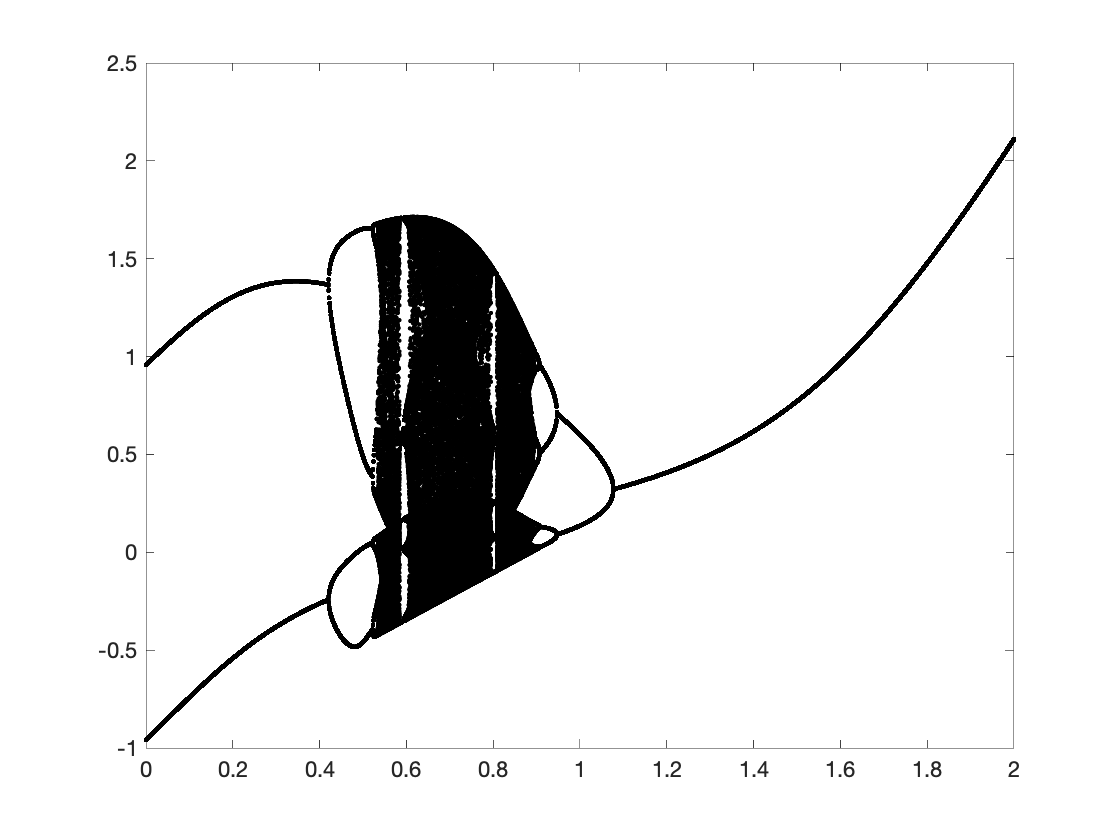
\includegraphics[width=0.7\textwidth]{pic81.png}
    \caption{使用chaos函数画出的分岔图}
\end{figure}

根据题目中的情景,我们仅考虑参数$c>0,q_t>0$的情况以符合实际意义。
通过更加细致的设定参数区间,我们得到了下图:
\begin{figure}[H]
    \centering
    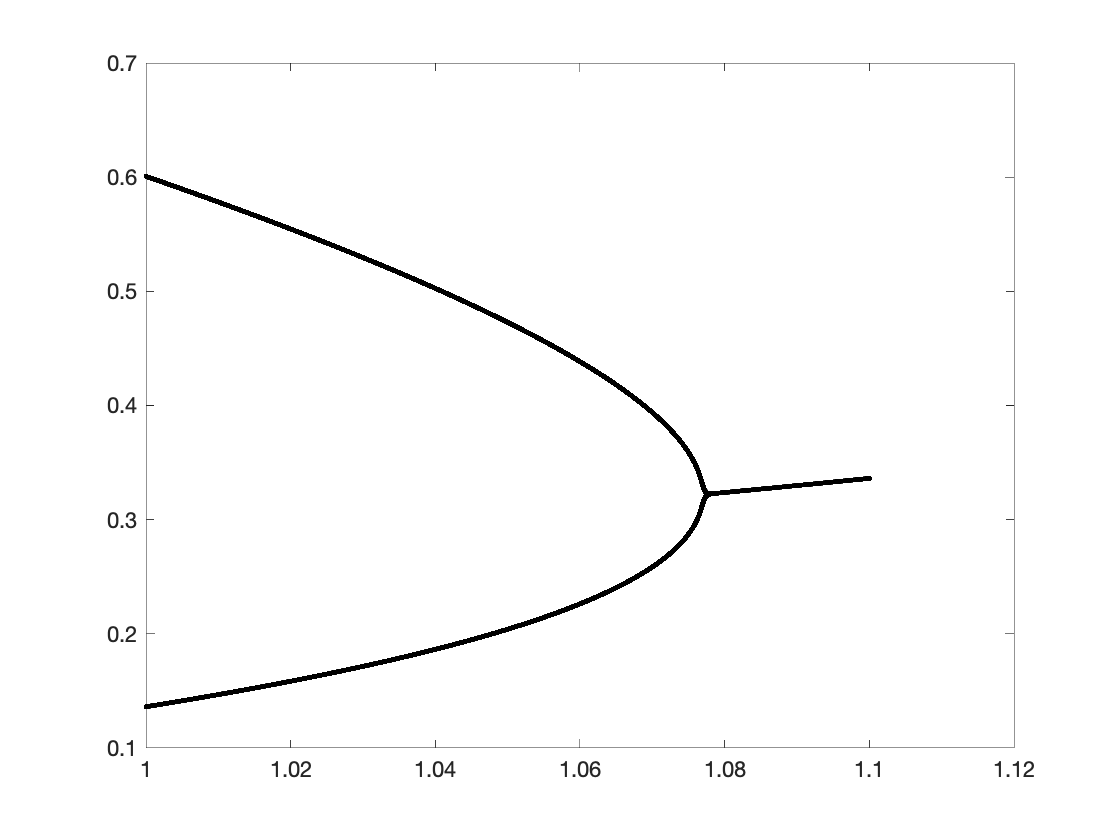
\includegraphics[width=0.7\textwidth]{pic82.png}
    \caption{第一个分岔点}
\end{figure}

\begin{figure}[H]
    \centering
    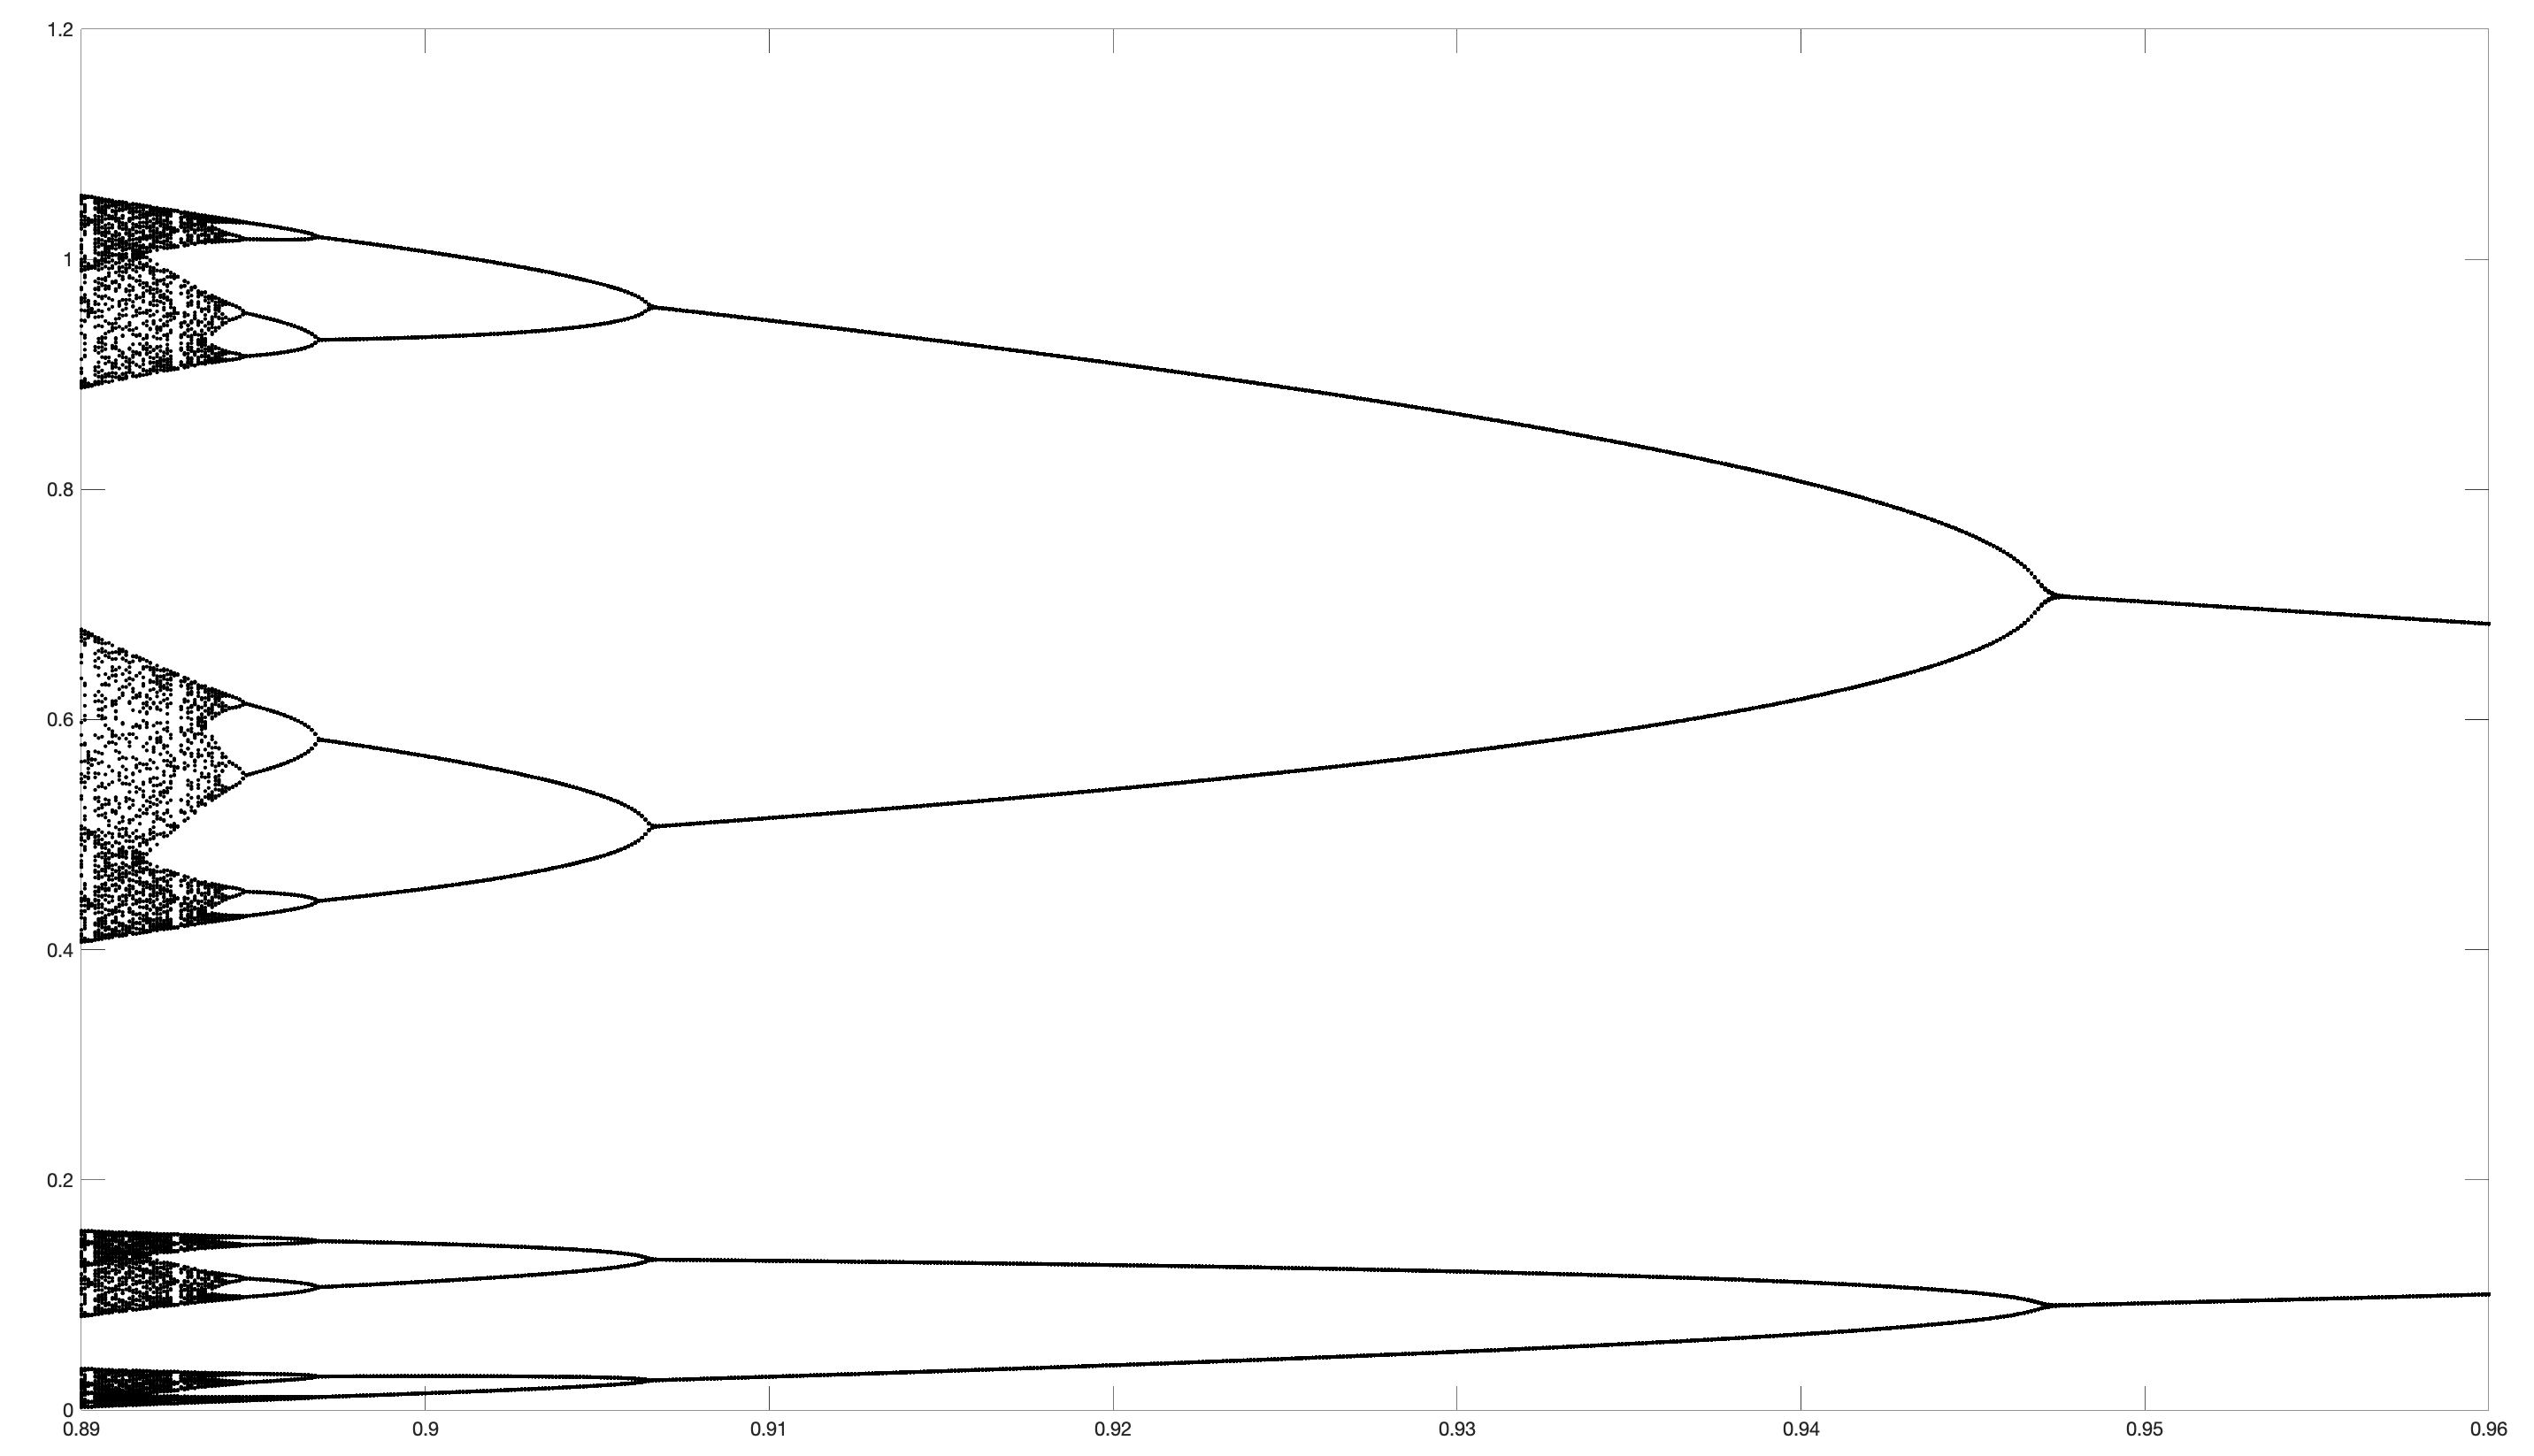
\includegraphics[width=1\textwidth]{pic84.png}
    \caption{其余分岔点}
\end{figure}

\begin{figure}[H]
    \centering
    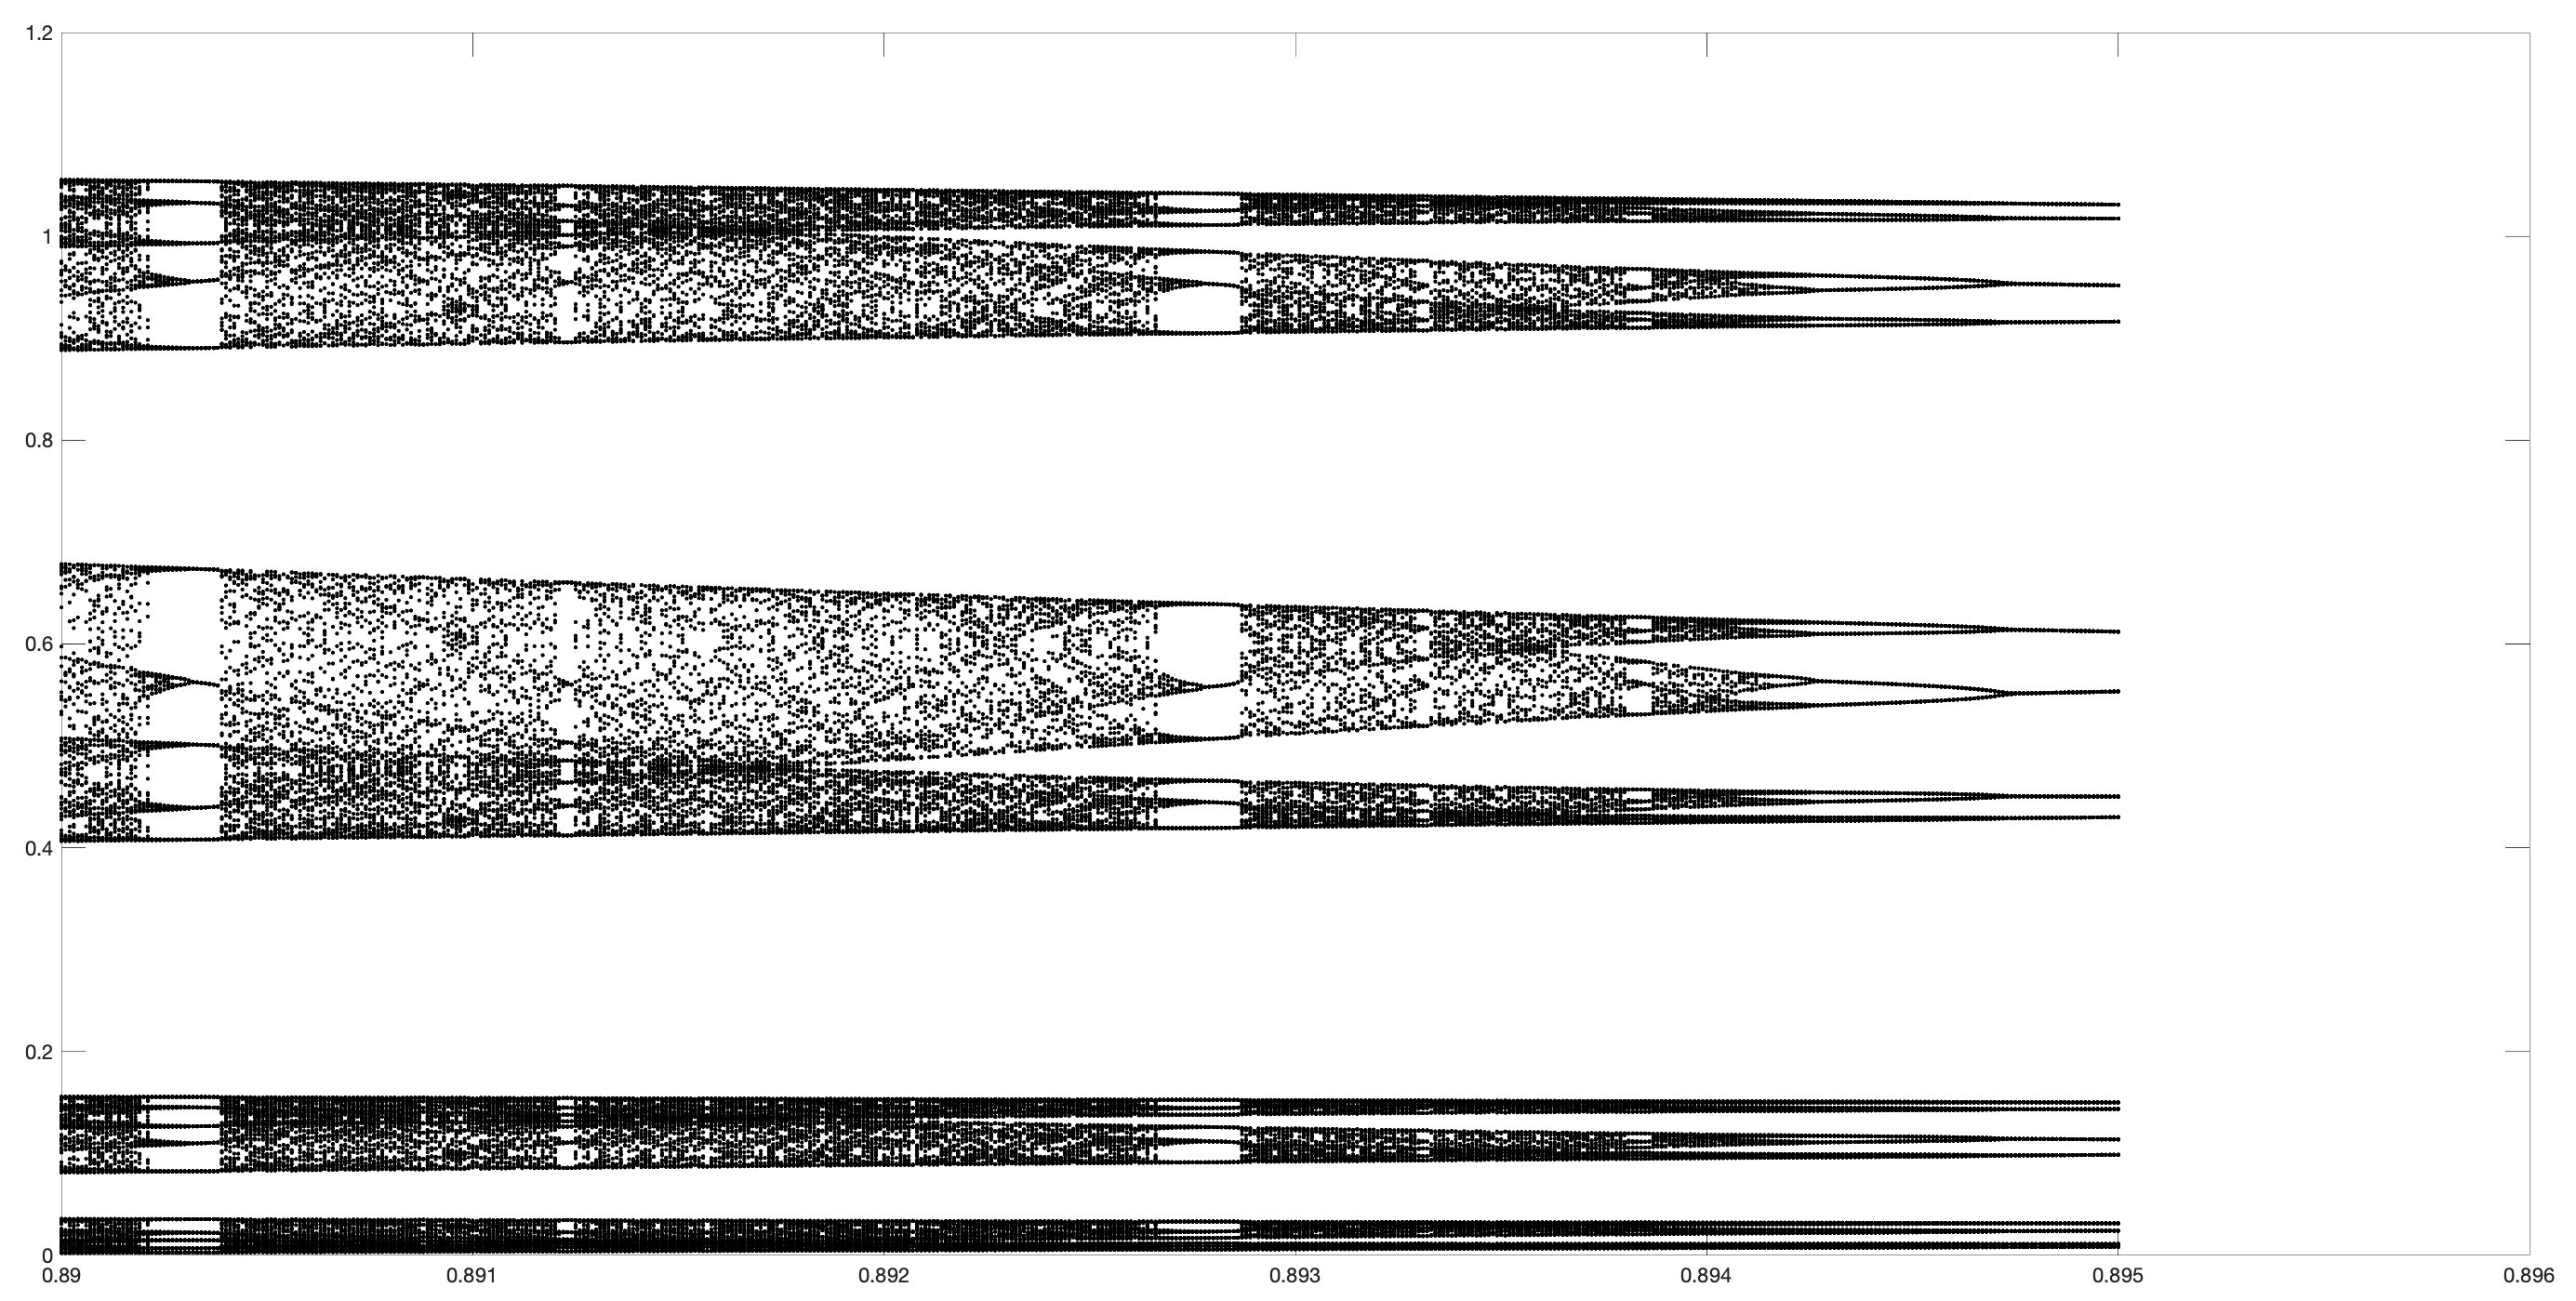
\includegraphics[width=1\textwidth]{pic85.png}
    \caption{当$c<0.88$时出现混沌现象}
\end{figure}

通过MATLAB代码可以求得分岔点的位置:

\begin{lstlisting}
%% Find Fork Point
find_fork(@qt, init_val, 1000, 1.0:0.0001:1.1, 0, 1e-7)
find_fork(@qt, init_val, 1000, 0.93:0.0001:0.96, 1, 1e-7)
find_fork(@qt, init_val, 1000, 0.90:0.0001:1.93, 2, 1e-7)
find_fork(@qt, init_val, 1000, 0.88:0.0001:0.90, 3, 1e-7)
find_fork(@qt, init_val, 1000, 0.88:0.0001:0.90, 4, 1e-7)
\end{lstlisting}

\begin{itemize}
    \item{第一个分岔点精确计算结果为$b_1=1.0800$}
    \item{第二个分岔点精确计算结果为$b_2=0.9492$}
    \item{第三个分岔点精确计算结果为$b_3=0.9075$}
    \item{第四个分岔点精确计算结果为$b_4=0.8973$}
    \item{第五个分岔点精确计算结果为$b_5=0.8949$}
\end{itemize}

当$c<0.88$的时候,已经不能观察出几个独立的明显的收敛序列了,出现了混沌现象。

计算:

$$\frac{b_2-b_1}{b_3-b_2}=3.13$$

$$\frac{b_3-b_2}{b_4-b_3}=4.09$$

$$\frac{b_4-b_3}{b_5-b_4}=4.25$$

可以看到,虽然本次实验中获得的$n$并不大,但是这三次的计算结果的发展趋势符合Feigenbahum常数定律,即$\frac{b_n-b_{n-1}}{b_{n+1}-b_n}$趋于4.67。

\section{收获和建议}

通过这次的实验,我对MATLAB中提供非线性方程组求解函数理解更加深刻,通过实际编程、画图的方式观察了方程求解的结果,这是书本上无法学到的知识。同时,在做上机实验的过程中,我对MATLAB这款软件的使用也更加熟练了。希望在之后的课堂上老师能够当堂进行相关的技巧演示并给出题目的分步解答。

\end{document}